%%%%%%%%%%%%%%%%%%%%%%%%%%%%%%%%%%%%%%%%%
% Beamer Presentation
% LaTeX Template
% Version 1.0 (10/11/12)
%
% This template has been downloaded from:
% http://www.LaTeXTemplates.com
%
% License:
% CC BY-NC-SA 3.0 (http://creativecommons.org/licenses/by-nc-sa/3.0/)
%
%%%%%%%%%%%%%%%%%%%%%%%%%%%%%%%%%%%%%%%%%

%----------------------------------------------------------------------------------------
%    PACKAGES AND THEMES
%-----------------------------------------z-----------------------------------------------

\documentclass[]{beamer}

\usepackage{amsfonts}
\usepackage{graphicx}
\usepackage{hyperref}
\usepackage{tabularx}
\usepackage{amsthm}
\usepackage[vcentermath]{youngtab}

\mode<presentation> {

\usetheme{CambridgeUS}

}

\setlength{\parskip}{1em}

\DeclareGraphicsExtensions{.pdf,.png,.jpg}

\newcommand{\btVFill}{\vskip0pt plus 1filll}

%----------------------------------------------------------------------------------------
%    TITLE PAGE
%----------------------------------------------------------------------------------------

\title[Why don't we have a quantum computer?]{Why don't we have a quantum computer (yet)?} % The short title appears at the bottom of every slide, the full title is only on the title page

\author[Alex E. Moylett]{Alex E. Moylett} % Your name
\institute[University of Bristol] % Your institution as it will appear on the bottom of every slide, may be shorthand to save space
{
Quantum Engineering Technology Labs and Quantum Engineering Centre for Doctoral Training\\
University of Bristol \\ % Your institution for the title page
\medskip
\textit{\href{mailto:alex.moylett@bristol.ac.uk}{alex.moylett@bristol.ac.uk}} % Your email address
}
\date{16th November 2017} % Date, can be changed to a custom date

\begin{document}

\begin{frame}
\titlepage % Print the title page as the first slide
\end{frame}

%----------------------------------------------------------------------------------------
%    PRESENTATION SLIDES
%----------------------------------------------------------------------------------------

%------------------------------------------------
\section{Quantum computers}
%------------------------------------------------

\begin{frame}
\frametitle{What is a quantum computer?}
A computer which uses the laws of quantum mechanics to solve some problems asymptotically faster than classical computers.
\end{frame}

\begin{frame}
\frametitle{Pros and cons of a quantum computer}

Pros:
\begin{itemize}
\item<2-> They push the limits of our best security protocols, via polynomial time algorithms for factoring and discrete log
\item<3-> They allow us to simulate scientific experiments exponentially faster
\item<4-> They can help us solve large search problems -- including NP-hard problems -- quadratically faster
\item<5-> They provide exponential speedups for some machine learning problems (SVM, PCA, recommendation systems)
\end{itemize}

Cons:
\begin{itemize}
\item<6-> They don't exist
\end{itemize}
\end{frame}

\begin{frame}[noframenumbering]
\frametitle{Pros and cons of a quantum computer}

Pros:
\begin{itemize}
\item They push the limits of our best security protocols, via polynomial time algorithms for factoring and discrete log
\item They allow us to simulate scientific experiments exponentially faster
\item They can help us solve large search problems -- including NP-hard problems -- quadratically faster
\item They provide exponential speedups for some machine learning problems (SVM, PCA, recommendation systems)
\end{itemize}

Cons:
\begin{itemize}
\item They don't exist(-ish)
\end{itemize}
\end{frame}

\begin{frame}
\frametitle{Do quantum computers exist?}

We do have quantum computers, including some which you can program on right now: \url{https://quantumexperience.ng.bluemix.net/qx}

The problem is that they are not currently large enough to outperform classical computers at the problems I mentioned earlier.

The largest number factorised by Shor's algorithm so far is 21\footnote{Martín-López et al., Nature Photonics, 6, 773}. Other quantum computing methods have achieved 291311\footnote{Li et al., {\tt arXiv:1706.08061}}, but this is still a way off breaking RSA.
\end{frame}

\section{D-Wave}

\begin{frame}
\frametitle{D-Wave 2000: The world's biggest quantum computer}

\begin{center}
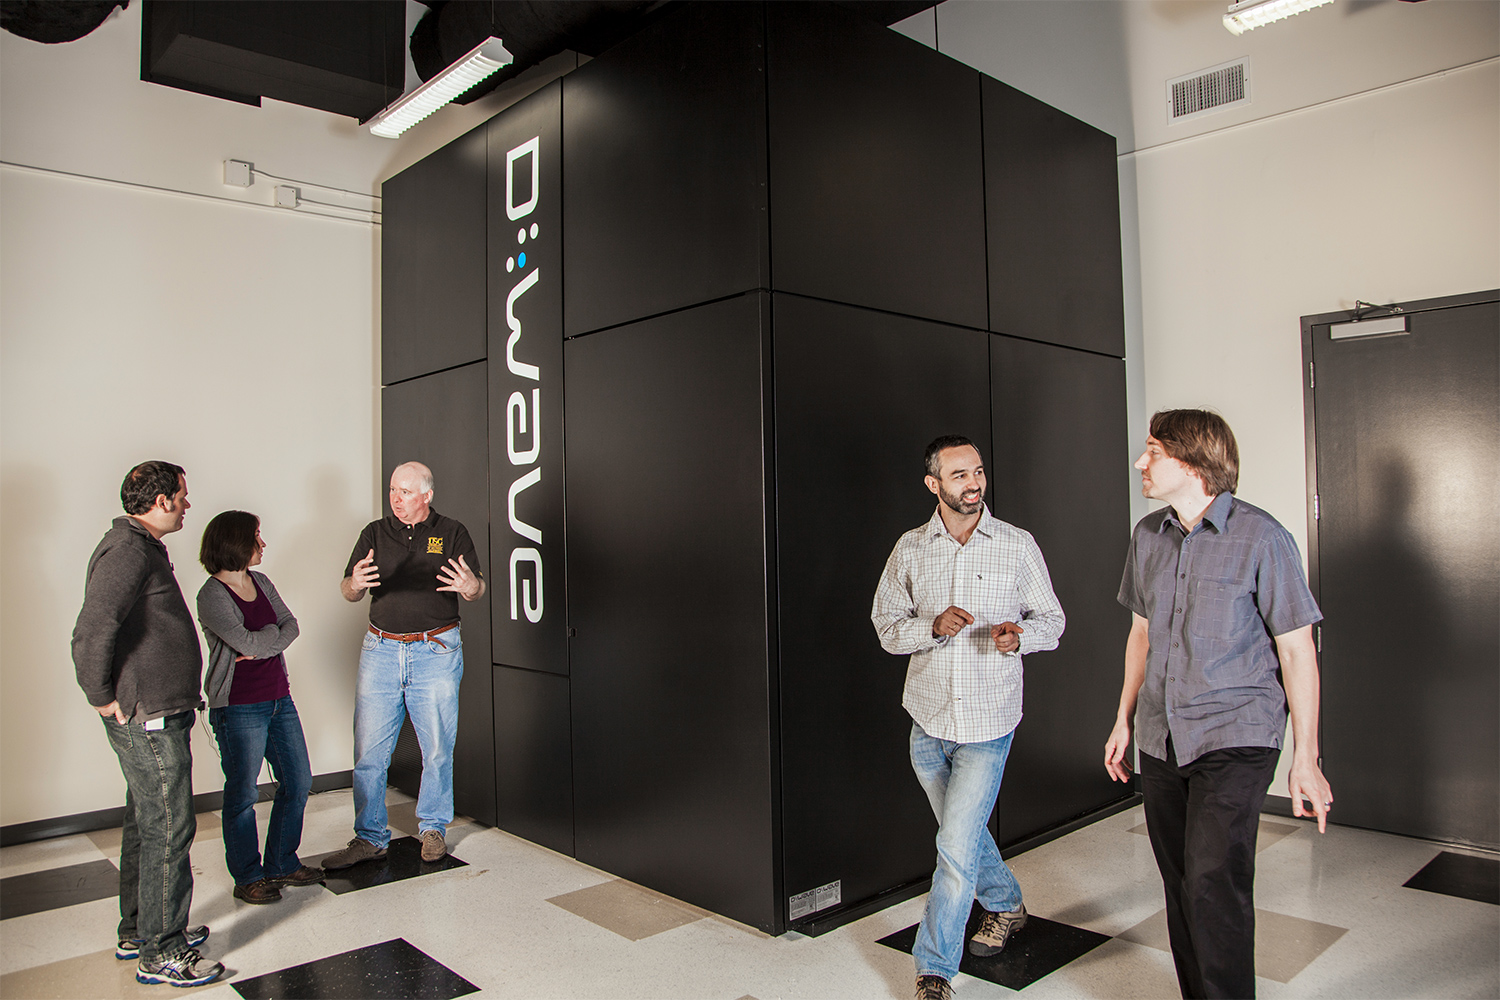
\includegraphics[scale=0.2]{dwave}
\end{center}
\end{frame}

\begin{frame}
\frametitle{How to access a D-Wave machine yourself!}

\begin{itemize}
\item<1-> Buy one yourself, for \$15 million\footnote{\url{https://www.wired.co.uk/article/d-wave-2000q-quantum-computer}}
\item<2-> Rent time on one, cheaper but still pricey
\item<3-> Use Selby's simulator, freely available on GitHub\footnote{\url{https://github.com/alex1770/QUBO-Chimera}}, demonstrated to run faster than earlier D-Wave machines and conjectured to be faster than the 2000Q\footnote{\url{http://www.archduke.org/stuff/d-wave-comment-on-comparison-with-classical-computers/harder-qubo-instances-on-a-chimera-graph/}}
\end{itemize}
\end{frame}

\begin{frame}
\frametitle{Quantum interference on a D-Wave machine}
\begin{center}
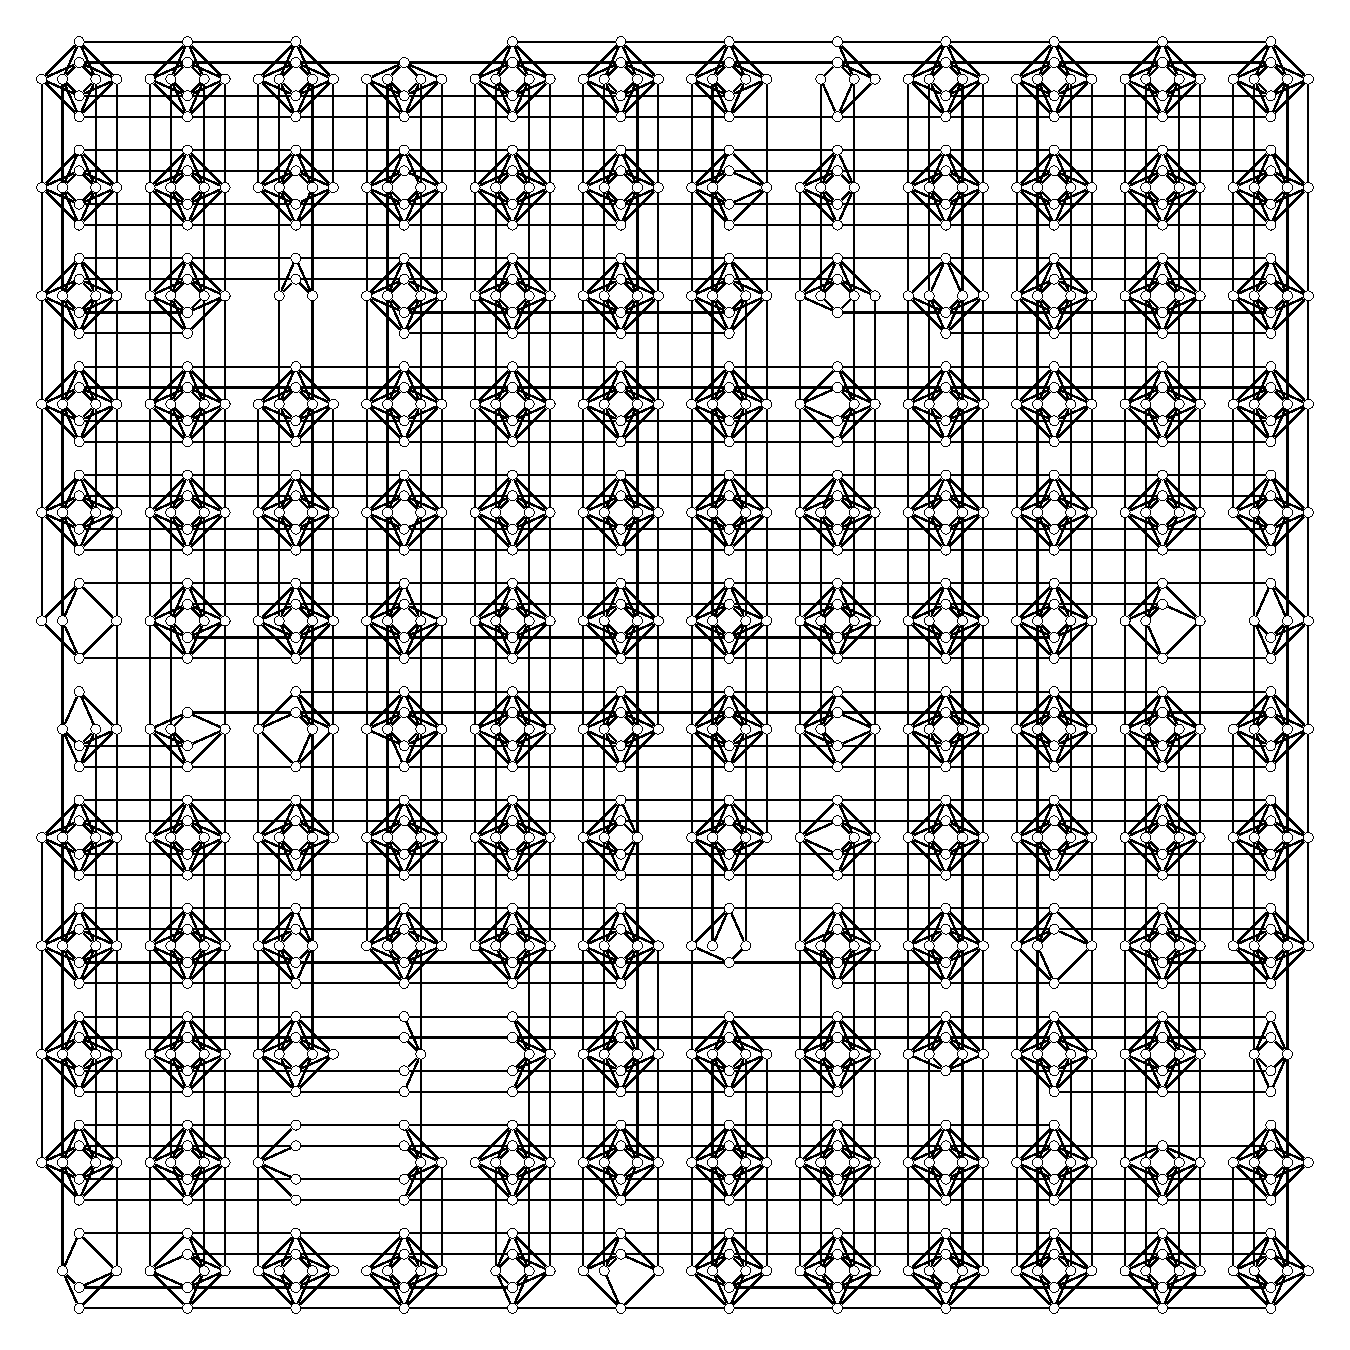
\includegraphics[scale=0.25]{dwave2x}\footnote{King et al., {\tt arXiv:1508.05087}}
\end{center}
\end{frame}

%------------------------------------------------
\section{Conclusion}
%------------------------------------------------

\begin{frame}
\frametitle{Conclusion}



\end{frame}

%------------------------------------------------
\section{And now a word from our sponsors!}
%------------------------------------------------

\begin{frame}
\frametitle{World Aids Day Red Run}

  \begin{columns}[T]
    \begin{column}{.5\textwidth}
    \begin{center}
    
\includegraphics[scale=0.4]{RR-logo}\\
    
\includegraphics[scale=0.7]{brigstowe}
    \end{center}
    \end{column}
    \begin{column}{.5\textwidth}
    \begin{itemize}
    \item I'm running ten kilometres
    
    \item Raising money for Brigstowe, \url{www.brigstowe.org}
    
    \item Please donate here \url{https://www.justgiving.com/fundraising/alex-moylett}
    
    \item Fancy dress suggestions appreciated!
    \end{itemize}
    \end{column}
  \end{columns}

\end{frame}

\begin{frame}
\frametitle{Quantum Engineering Centre for Doctoral Training}

  \begin{columns}[T]
    \begin{column}{.5\textwidth}
    \begin{center}
    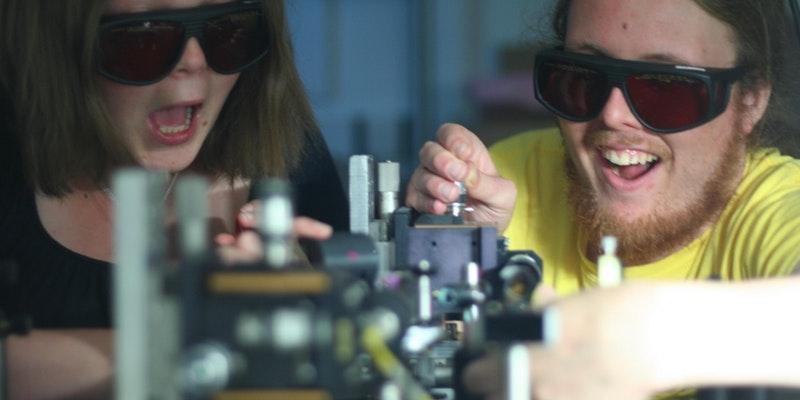
\includegraphics[scale=0.2]{cdt_open_day}
    \end{center}
    \end{column}
    \begin{column}{.5\textwidth}
    \begin{itemize}
    \item 1 year MRes including experimental, theoretical and taught work, plus 3 year PhD on a research project of your choice
    
    \item Fully funded
    
    \item Opportunities to travel and collaborate with other researchers in academia and industry
    \end{itemize}
    \end{column}
  \end{columns}
  
  Open day 5th December: \url{https://www.eventbrite.co.uk/e/quantum-engineering-bristol-tickets-39609797972}

\end{frame}

%------------------------------------------------
\section{The End}
%------------------------------------------------

\begin{frame}
\frametitle{The end}
\begin{center}
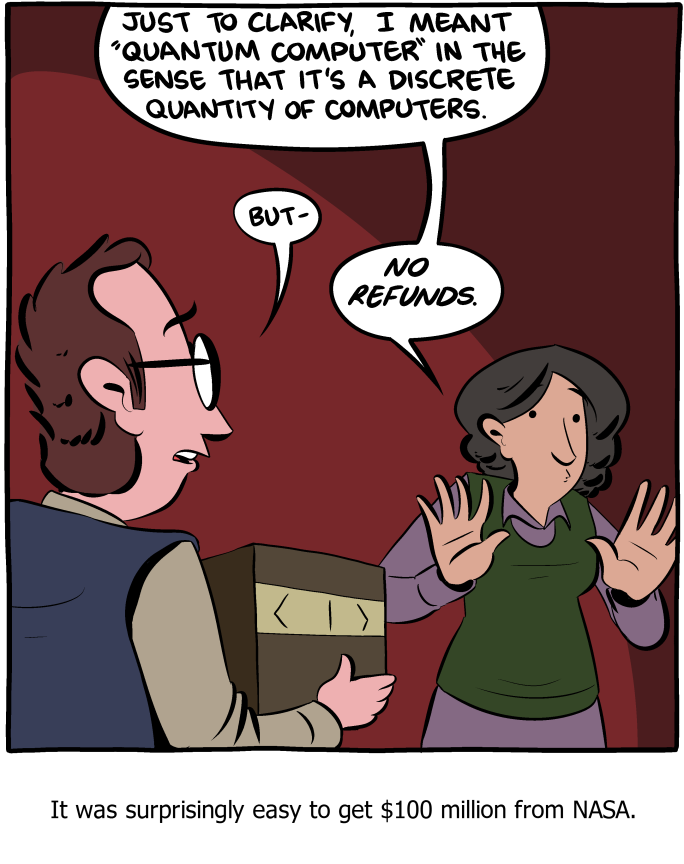
\includegraphics[scale=0.2]{smbc}\footnote{\url{http://www.smbc-comics.com/comic/quantum-computer}}

Any questions?
\end{center}
\end{frame}

%------------------------------------------------
\section{Post-credits}
%------------------------------------------------

\begin{frame}[noframenumbering]
\frametitle{Post-credits}
This is the third time I've done one of these post-credit slides. A hat trick of useless slides!
\end{frame}

%----------------------------------------------------------------------------------------

\end{document} 
